\section{Design and Implementation of \textsf{PCStream}}
In this section, we describe in detail the proposed automatic stream management technique,
\textsf{\small PCStream}.  We first explain how we automatically extract PCs during
runtime and describe how multiple PCs are mapped to streams in an SSD.

Fig.~\ref{fig:architecture} shows an overall organization of \textsf{\small PCStream}.
\textit{The PC extractor module}, which is implemented in the Linux kernel as
part of a system call handler, 
computes a PC signature, which is used as a unique ID for each program context.  
We use the signature program counter~\cite{PC} as a PC signature 
by summing program counter values along the execution path to a write-related system function 
(e.g., {\tt write()}).  
With the PC signature, we can monitor the data lifetime of each write at the program context level. 
A PC signature value is stored
in an inode data structure of a file system (modified for \textsf{\small PCStream})
and is delivered to \textit{the lifetime analyzer module} which estimates
expected lifetimes of data belonging to a given PC in the block device level.
In order to efficiently detect the end of data lifetime in append-only
workloads, the lifetime analyzer also intercepts TRIM~\cite{TRIM} requests from a file system.  %shane part
Based on the lifetime information, \textit{the PC-to-stream
mapper module} clusters PCs with similar lifetimes and maps them together to
the same stream ID.  This mapping is required because 
the number of streams in an SSD is generally less than the number of PCs in host applications.

\subsection{Automatic PC computation}
As mentioned earlier, a PC is represented by a PC signature which is defined as
the sum of program counter values along the execution path of a function call that
finally reaches a write-related system function. A function call involves
pushing the next program counter, which is used as a return address, to the
stack followed by pushing a frame pointer value.  In general, by using frame
pointer values, we are able to back-track the stack frames of the process and
selectively get return addresses for generating a PC signature.  For example,
Fig.~\ref{fig:getpc}(a) shows the abstracted execution path for flushing data
in RocksDB and Fig.~\ref{fig:getpc}(b) illustrates how a PC signature is obtained
by back-tracking the stack.  
Since a frame pointer value in the stack holds the address of the previous
frame pointer, the PC extractor can easily obtain return addresses and
accumulate them to compute a PC signature. 
(The return addresses are pushed
before calling the \textsf{\small  write()}, \textsf{\small  BuildTable()} and \textsf{\small 
WriteLevel0Table()} functions.)

\begin{figure}[t]
	\centering
	%\vspace{-10pt}
	%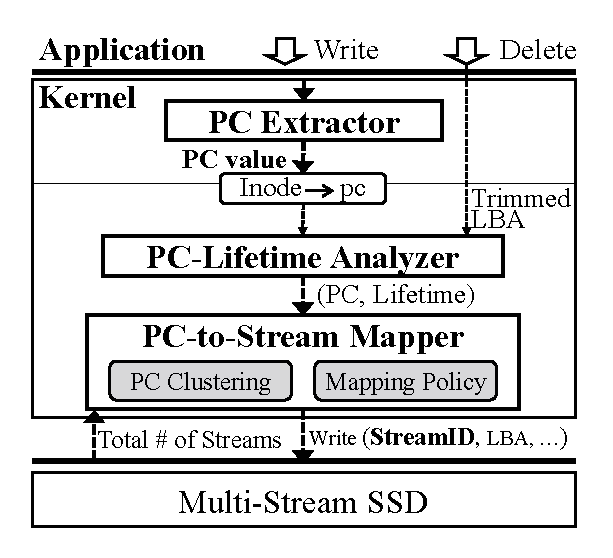
\includegraphics[width=0.6\linewidth]{figure/architecture4}
	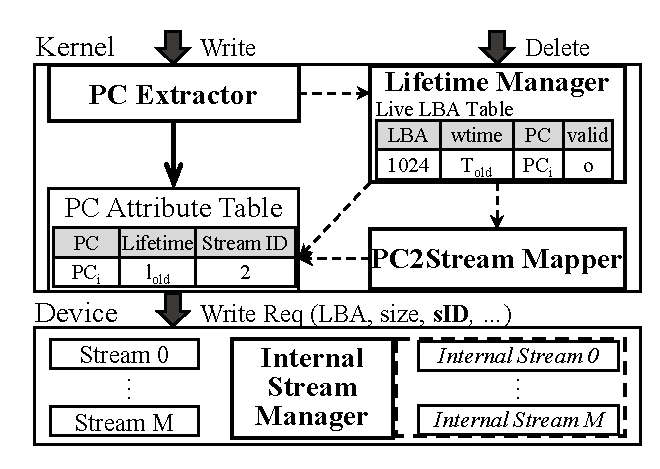
\includegraphics[width=0.6\linewidth]{figure/overview}
	%\vspace{-9pt}
	\caption{An overall architecture of \textsf{\small PCStream}.}
	\label{fig:architecture}
	%\vspace{-22pt}
\end{figure}


The frame pointer-based approach for computing PC signatures, however, is not
always possible because modern C/C++ compilers often do not use the frame
pointer for improving the efficiency of register allocation.
One example is a
{\tt -fomit-frame-pointer} option of GCC~\cite{GCC}. 
Although this option allows the frame pointer to be used as a general-purpose
register for high performance, it makes very difficult for us to back-track
return addresses along the call chains.  

\begin{figure}[b]
%	\vspace{-10pt}
	\centering
	%\vspace{-8pt}
	\subfloat[An abstracted execution path for flushing data.]{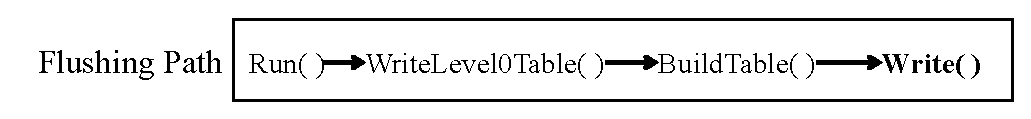
\includegraphics[width=0.4\textwidth]{figure/getpc_1}}  
	%\vspace{-14pt}
	\hfill
	\subfloat[with the frame pointer.]{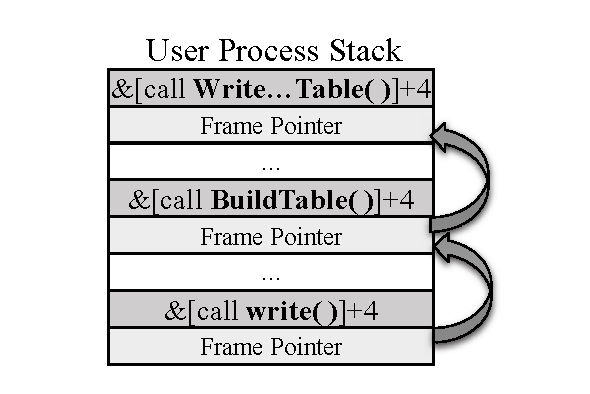
\includegraphics[width=0.22\textwidth]{figure/getpc_2}}
	\subfloat[without the frame pointer.]{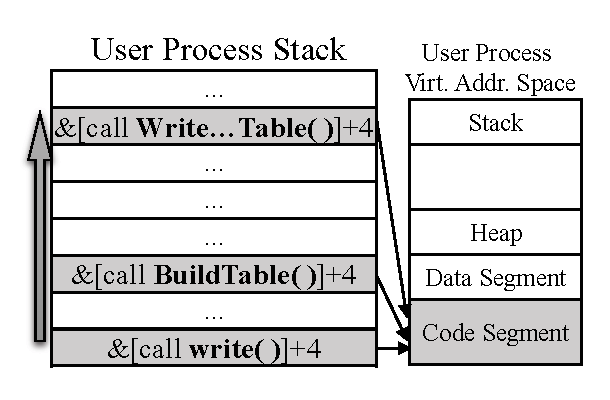
\includegraphics[width=0.22\textwidth]{figure/getpc_3}}
	%\vspace{-9pt}
	%\caption{An example execution path and its PC extraction methods.}
	\caption{An example execution path and its PC extraction.} %shane part
	\label{fig:getpc}
	%\vspace{-20pt}
\end{figure}

In \textsf{\small PCStream}, we employ a simple but effective workaround 
for backtracking the call stack when the frame pointer is not used.
When a write system call is made, we scan every word in the stack and check
if it belongs to the process's code segment.  If the scanned stack word holds a
value within the address range of the code segment, we assume that it is a
return address.  Since scanning the full stack takes too long, we stop the
stack scanning procedure when a sufficient number of return address candidates
are found.  In the current version, we stop when 5 return address candidates
are found.  Although quite ad-hoc, a restricted scan is effective in
distinguishing different PCs because two different PCs
cannot follow the same execution path to write system functions.  
(If they do, they are the same PC.) In our evaluation
with a 3.4 GHz CPU machine, the performance overhead of the restricted scan was
almost negligible, taking only 300-400 $n$sec per write system call.

\subsection{PC extraction for indirect writes}
{\color{blue}
앞서 언급한 방식은 write system call을 직접 호출하는 응용에 효과적이지만,
write system call을 직접 호출하지 않고 indirect write을 하는 응용에 대해서는 효과가 없다.
예를 들어, cassandra와 같이 JVM 기반의 응용은 write system call을 직접 호출하는 대신, Java가 제공하는 interface
를 사용하여 간접적으로 쓰기를 수행 한다.
이 경우, write system call 수준에서 PC를 추출하면, JVM 상에서 어떤 응용이 수행되고 있는지와는 관계없이 Java의
I/O를 담당하는 프로세스의 call stack만을 얻기 때문에 응용 프로그램의 I/O activity를 구분하려는 목적을 달성할 수 없다.
이러한 문제를 해결하기 위해서는 데이터가 만들어진 context를 정확히 파악할 수 있는 layer에서 PC가 계산 되어야 한다.
위의 예시에서는, system call layer 대신 Java interface를 통해 쓰기 요청을 전달 받을 때, PC extractor를 수행하면 의미있는
I/O activity를 구분할 수 있고 우리는 JDK를 수정하여 이러한 접근이 동작함을 확인하였다.
또 다른 indirect write case로, 프로그램 내부에 buffer를 유지하면서 이를 flushing하는 별도의 thread가 존재하는 경우가 있다.
이 역시 I/O activity를 구분할 수 있는 buffer에 데이터를 기록하는 시점에 구분되기 때문에, system call layer에서 PC를 추출하면 
의미 없는 flushing thread의 call stack만을 얻게 된다. 
그러나 이 case는 I/O activity가 구분되는 지점이 프로그램 내부의 function call로 이루어지기 때문에 프로그램이 이를 
알려주지 않는 이상 system 수준에서 이를 직접적으로 파악하기 어렵다. 
프로그램을 수정하지 않고 buffering의 I/O activity를 구분하는 문제는 이 논문에서 다루기에는
너무 복잡하기 때문에 future work으로 남긴다.
}

\subsection{PC lifetime management}
{\color{blue}Lifetime manager는 생성된 데이터의 수명을 계산하고 이를 PC 별로 구분하여 관리한다.
Lifetime Manager의 목적은 PC별 수명의 패턴을 파악하여 stream 할당의 기준을 만드는 것이다.
다양한 평가 결과, 우리는 동일한 I/O activity의 데이터라도 update 혹은 삭제 시기에 따라
개별적 데이터의 수명은 조금씩 달라지지만, 고유한 수명 패턴은 유지되는 것을 확인하였다.
따라서 lifetime manager는 수명의 정확한 값을 추구하기 보다는 수명의 대략적인 패턴을 파악하는 것을 목표로 한다.

데이터 lifetime은 쓰기 request가 issue된 때 부터 해당 주소가 다시 write되거나 
TRIM command에 의해 삭제될 때 까지로 정의된다.}
%The data lifetime of the append-only workload is defined 
%from when a write request is issued until the TRIM command~\cite{TRIM} is issued to 
%the corresponding address.
In order to measure the lifetime of data, the lifetime analyzer 
records the write time and PC value for each write request using its LBA.
Upon receiving the TRIM command or updating write request, the lifetime analyzer can compute the 
lifetime of the corresponding data using the recorded information.
{\color{blue} 
그러나 device 전체 LBA 공간에 대해 쓰여진 시간 정보를 유지하는 것은 메모리 부하가 크기 때문에,
우리는 1MB 크기의 chunk 단위로 나누어 관리하는 최적화 기법을 사용한다.
}
Note that, the
same PC may generate multiple data streams with different lifetimes.
We take the average lifetime as the PC's lifetime.

{\color{blue} Section 3에서 언급했듯이, PC는 user stack에 존재하는 
return address 즉, virtual address 기반으로 계산되므로
한 프로그램을 반복적으로 수행하면 동일한 PC들을 발견할 수 있다.
첫번째 수행 중 얻은 PC 별 lifetime 정보를 다음번 수행에서도 활용하기 위해 
이 정보를 유지하는 cache를 사용한다.
등장한 PC들과 그들의 lifetime 정보는 cache에 유지되고 추후 동일한 PC에 대해서는 
누적된 수명 정보를 활용할 수 있기 때문에 좀 더 정확한 수명 판단이 가능하다.
PC 값과 수명 값의 크기가 작기 때문에 몇십 KB의 메모리 만으로 충분히 많은 양의 데이터를 
유지할 수 있다. 따라서 본 논문에서는 PC cache replacement 정책에 대해서는 논의하지 않는다.
}

\subsection{Mapping PCs to SSD streams}

The last step in \textsf{\small PCStream} is to map
a group of PCs with similar lifetimes to an SSD stream.
This is because each SSD supports a limited number of stream IDs. For
example, SSDs used in \textsf{\small FStream}~\cite{FStream} and \textsf{\small AutoStream}~\cite{AutoStream}
support only 9 and 16 streams, respectively. 
{\color{blue} PC cluster는 비슷한 수준의 수명을 가진 PC들을 하나의 group으로 구분하기 위해 clustering algorithm을 사용한다.
본 연구에서는 overhead가 적고 많이 사용되는 k-means 알고리즘을 사용하였다.
SSD가 제공하는 stream의 개수와 동일한 group을 생성하여 각 PC group을 각 stream으로 할당한다.
}

%To properly group multiple PCs,
%the PC-to-stream mapper employs a simple 1-D clustering algorithm. 
%In order to cluster PCs with similar lifetimes, the mapper calculates the 
%lifetime difference between PCs.
%Then, PCs with the smallest lifetime difference are clustered into the same PC group. 
%The mapper repeats this clustering step until all the PCs are assigned to their PC groups.
{\color{blue} 추가로, SSD가 지원하는 stream의 개수가 변경되는 상황에서도 reclustering을 통해
대응이 가능하다.
For adapting to changing workloads, reclustering operations should be regularly performed. 
reclustering의 주기는 workload의 변화 패턴에 따라 결정될 수 있다.
새로운 PC가 계속적으로 생성되거나 한 PC의 수명 패턴이 자주 변화할 경우 reclustering의 주기를 
좀 더 짧게 설정하여 workload 변화를 반영한다.
}
%Since the
%number of PCs created by applications is not limited, the clustering algorithm
%must be efficient enough to quickly handle many PCs. 


